% The entire content of this work (including the source code
% for TeX files and the generated PDF documents) by 
% Hongxiang Chen (nicknamed we.taper, or just Taper) is
% licensed under a 
% Creative Commons Attribution-NonCommercial-ShareAlike 4.0 
% International License (Link to the complete license text:
% http://creativecommons.org/licenses/by-nc-sa/4.0/).
\documentclass{article}

% My own physics package
% The following line load the package xparse with additional option to
% prevent the annoying warnings, which are caused by the package
% "physics" loaded in package "physicist-taper".
\usepackage[log-declarations=false]{xparse}
\usepackage{physicist-taper}
\makenomenclature % For an index of symbols.

\usepackage{menukeys}
\newcommand\command[1]{\texttt{\centering #1}}

\title{Installation Guides}
\date{\today}
\author{Taper}


\begin{document}


\maketitle
\abstract{
This document installs the necessary software and plugins for
\href{https://github.com/lervag/vimtex}{Vimtex} on a windows machine.
It uses a \texttt{vimrc} written by myself to free user from
configuration.  However, it does not explains the details of that
\texttt{vimrc}.
}    
\tableofcontents

\section{List of software to be installed}
\label{sec:list of software}

\begin{enumerate}
    \item \TeX Live 2016 (\texttt{textlive2016-20160523.iso}).
    \item Vim, as in gVim
        (The latest 32bit (v8.0.0540)
        \href{https://github.com/vim/vim-win32-installer/releases/}{here}
        which has \texttt{Lua} support enabled.).
    \item Git (v2.12.2 64bit).
    \item SumatraPDF (v3.1.2 64bit).
    \item Texstudio (v2.12.2).
    \item Python (v2.7.13 32bit).
    \item Notepad++ (v7.3.3).
    \item Vundle (latest commit on
        \href{https://github.com/VundleVim/Vundle.vim}{Github
        Vundle}), and many related plugins for Vim.
\end{enumerate}

\section{Install Steps}
\label{sec:Install Steps}

\begin{enumerate}
    \item \TeX Live.

        First mount the ISO file (double click in Windows 8 or later,
        use third-part software in Windows 7 or earlier). Then open
        the file \texttt{install-tl-windows.bat}, and install with all
        default settings (except that you may want to change the
        installation folder).

        The installation will take a lot of time. Continue to the next
        steps while waiting for this \TeX Live installation to finish.

        \textbf{Explanation}: \TeX Live provides us with basic \TeX
        utilities and packages. Although it is big, the exhaustive
        packages it provides will be handy when we write \LaTeX{} daily.

    \item Install the gVim. As mentioned, \textbf{DO NOT} install the
        version downloaded from the Vim project's website. Use the
        link
        \href{https://github.com/vim/vim-win32-installer/releases/}{here}
        to download the version which has \texttt{Lua} support
        enabled. Install with default configuration, except that you 
        will need to consider the following options:

        In this figure:
        \begin{figure}[H]
            \centering
            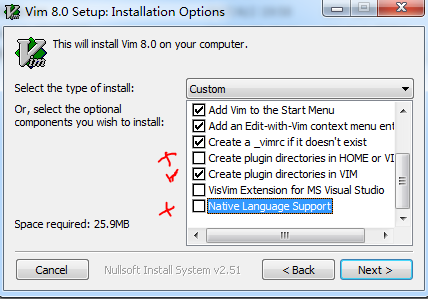
\includegraphics[width=0.6\linewidth]{pics/1.PNG}
        \end{figure}
        I encourage you
        \footnote{And if you do not follow my suggestion, you might
            need extra modification to my \texttt{vimrc} file.}
        to disable \menu{Create plugin directories in
        \texttt{HOME} or \texttt{VIM}}, and enable instead \menu{
        Create plugin directories in \texttt{VIM}}.  This make Vim put
        its plugin directory inside \texttt{VIM} folder (which is the
        folder where \texttt{VIM}) is installed.  Therefore, the Vim
        plugins would not mess up inside your \texttt{HOME} folder
        (which on Windows, people seldom touches upon), and Vim
        becomes more portable.

        I also encourage you to disable \menu{Native Language
        Support}, which force us to speak in English with Vim.

        \textbf{Explanation}: gVim will be our editor. And
        \texttt{Lua} will provide support for some plugins of Vim.

    \item Add Vim to system \texttt{PATH} variable, just like what you
        have done when installing \texttt{Java}.
    \item Add Lua Support for Vim. Download
        \href{http://luabinaries.sourceforge.net/download.html}{Lua
        Binary}. The version of Lua should be consistent with the Vim
        (gVim) you installed (same OS, same architecture), and those
        DLL with MingW support are not required
        \footnote{Actually I never tested those with MingW support.
        Therefore, I do not recommand trying them.}.

        After downloading, extra the compressed file and copy the file
        \texttt{lua53.dll} \footnote{the number 53 for version may be different
        in your case. But it is the DLL file that we cared about.} and
        move it to \path{Folder Where Vim Is Installed> vim80}
        \footnote{The number $80$ is the version number of vim.} like
        this:
        \begin{figure}[H]
            \centering
            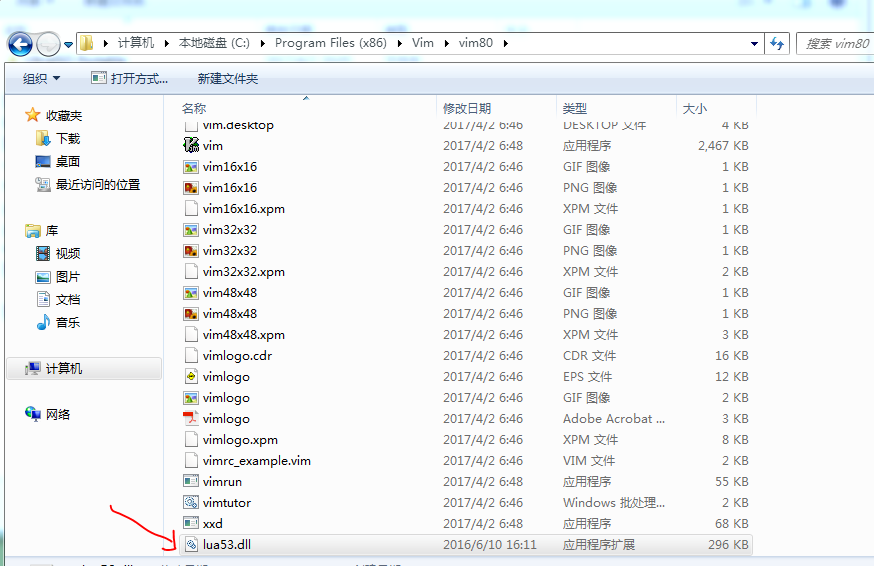
\includegraphics[width=0.6\linewidth]{pics/8.PNG}
        \end{figure}

    \item Install Git, with mostly default option, except that you
        should change the default installation folder to somewhere you
        like.

        \textbf{Explanation}: Git will be used to download Vim plugins
        from GitHub.

    \item Install SumatraPDF viewer, which is the only viewer that can
        cooperate with \texttt{vimtex} plugin and support re-rendering
        of PDF once a change is made to the PDF file. Add SumatraPDF
        to your system's \texttt{PATH} variable.

        Configuration of SumatraPDF: \newline
        Set the the \menu{inverse search command-line} to this value:
        \begin{lstlisting}
            gvim --remote-silent +%l "%f"
        \end{lstlisting}
    \item Install \TeX{} Studio, with default configuration, to folder
        where you prefer. 

        \textbf{Explanation}: \TeX{} Studio provides very useful list
        of commands, reference tables for editing \LaTeX.

    \item Install \texttt{Python} with mostly default configuration. Note
        that you should add \texttt{Python} to the system
        \texttt{PATH} variable too:
        \begin{figure}[H]
            \centering
            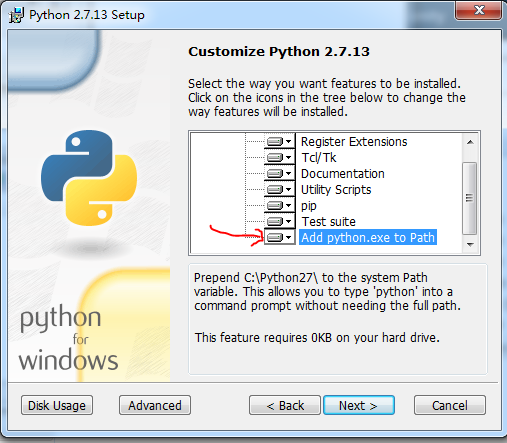
\includegraphics[width=0.6\linewidth]{pics/3.PNG}
        \end{figure}

    \item Install a handy but advanced (better than Notepad) text
        editor. I prefer Notepad++ for its small file size.
    \item Set up Vim configuration, and some Vim plugins. Vundle is
        the first and most important Vim plugin that manages other
        plugins (a plugin that manages plugins). Installation is
        straight forward. 
        
        \begin{enumerate}
            \item Clone it with git to somewhere you like:

                \texttt{\footnotesize git clone
                https://github.com/VundleVim/Vundle.vim.git}
            \item Move the downloaded folder to
                \path{Vim Installation Folder > vimfiles > bundle >
                Vundle.vim} (create new empty folder is required).
            \item  Copy my configuration text to file \texttt{\_vimrc},
                which can be found in the folder \path{where Vim is
                installed}. My configuration text can be found here:
                \href{https://github.com/we-taper/vimConfig/blob/master/_vimrc}
                {My GitHub Link}.

            \item Modify some part of my configuration to suit your
                compter setup:
                \begin{itemize}
                    \item Before you actually install the color scheme
                        for Vim, disable it first. You will find this line:

                        \command{ colorscheme~Atelier\_SulphurpoolDark }

                        And add double quote mark at the beginning to
                        comment it out.
                    \item Let Vim find python properly. You will find
                        a line starts with \menu{let \$PYTHONPATH=},
                        followed by some path, and you should change
                        all of them to the correct path to locate the
                        python files you installed.
                    \item Disable the font I set. Since you should
                        have not yet installed my font, disable the
                        setting first. This is done by comment out the
                        code within a if statement: \menu{if
                        has('gui\_running')}.
                \end{itemize}
        \end{enumerate}
        
\end{enumerate}
% \bibliography{cite}{}
% \bibliographystyle{alphaurl}

% \begin{thebibliography}{1}
% 	\bibitem{book} 
% \end{thebibliography}
\printnomenclature
\section{License}
The entire content of this work (including the source code
for TeX files and the generated PDF documents) by 
Hongxiang Chen (nicknamed we.taper, or just Taper) is
licensed under a 
\href{http://creativecommons.org/licenses/by-nc-sa/4.0/}{Creative 
Commons Attribution-NonCommercial-ShareAlike 4.0 International 
License}. Permissions beyond the scope of this 
license may be available at 
\href{http://www.google.com/recaptcha/mailhide/d?k=015LguzBJigi0rpyuJRqLoig==\&c=p1c-M-mm7ZcjUCkTuZZa9eEPHRVk6paN0694iazlQy8=}
{[My Email Address(Click)]}.
\end{document}
